\documentclass[11pt]{article}

\usepackage[a4paper,margin=1in]{geometry}
\usepackage{amsmath,amssymb}
\usepackage{booktabs}
\usepackage{array}
\usepackage{xcolor}
\usepackage{microtype}
\usepackage{hyperref}
\usepackage{url}
\usepackage{pgfplots}
\pgfplotsset{compat=1.18}
\usetikzlibrary{positioning}


% Allow \path/\url to break long hexadecimal hashes at any character
\makeatletter
\def\UrlBreaks{\do\/\do\a\do\b\do\c\do\d\do\e\do\f\do\0\do\1\do\2\do\3\do\4\do\5\do\6\do\7\do\8\do\9\do\.\do\@\do\!\do\_\do\|\do\;\do\>\do\]\do\)\do\,\do\?\do\'\do\+\do\=\do\#\do\-\do\:\do\~}
\makeatother

\hypersetup{
  colorlinks=true,
  linkcolor=blue!55!black,
  citecolor=blue!55!black,
  urlcolor=blue!65!black
}

\newcommand{\pL}{p_{\mathrm L}}
\newcommand{\RR}{\mathbb{R}}
\newcommand{\F}{\mathcal{F}}

\title{\textbf{Response-Fibre Schedule Optimization Lowers the Minimum Tested Surface-Code Distance in a Synthetic Fault Model:}\\
A Prospective Fixed-Reliability Audit}

\author{Y.Y.N. Li\\
\small Independent Researcher}

\date{}

\begin{document}

\maketitle

\begin{abstract}
Can schedule freedom, while preserving a declared affine mean-one response, reduce the minimum tested code distance at fixed logical reliability? Using a projected geometric flow that preserves a rowwise mean-one schedule constraint while minimizing a synthetic exposure score, we prospectively audit a rotated surface-code memory model. On three frozen prospective seeds, the optimized schedule reduces the minimum tested distance satisfying the frozen Wilson criterion at target \(\pL \le 0.025\) from \(d=11\) to \(d=9\), saving 45.3\% in the declared active-coordinate qubit-round proxy. The schedule-to-fault map is synthetic, and no hardware is tested; the result is therefore a prospective numerical mechanism inside the specified model, not a threshold or hardware claim.
\end{abstract}

\section{Introduction}

Many compiler benchmarks are summarized by a scalar gate-error metric, whereas quantum error correction (QEC) performance can depend on the full location- and correlation-resolved detector error model. Compilation and QEC are often evaluated at different abstraction levels; this separation assumes that the compiler is merely a black box that lowers the physical error rate \(p\).

We challenge this decoupling at the scheduling level with a single question: \textbf{Can schedule freedom, while preserving a declared affine response, reduce the minimum tested distance satisfying the frozen criterion at fixed logical reliability?} Multiple schedules can preserve the same declared affine constraint but expose qubits to different time-dependent correlations. In a surface code, these correlations enter the syndrome graph as edge-weight variations and are not captured by a single infidelity figure.

We express this freedom as a response fibre \(\F_c\)---the set of all schedules that share a declared affine response \(c\). A projected geometric flow on this fibre preserves the response while reshaping the fault correlation structure via projection of the negative exposure gradient onto the fibre tangent space (Eq.~\eqref{eq:general-flow}), with backtracking to enforce the box constraints. This separates the response (what schedule constraint must remain unchanged) from the exposure (how it is realized).

We do not prove a general theorem. Instead, we give a fail-closed numerical audit in an explicit setting: a rotated-surface-code memory, Stim circuits~\cite{Gidney2021}, and PyMatching decoding~\cite{Higgott2022}. The design score is evaluated before stochastic simulation; all claims are decided from Monte Carlo outcomes held out from optimization, although the design and evaluation share the frozen analytic schedule-to-fault map. On a frozen prospective cohort, at target \(\pL=0.025\), all three seeds exhibit a minimum tested-distance crossover from \(d=11\) to \(d=9\), corresponding to a 45.3\% reduction in the declared active-coordinate qubit-round proxy. The supported claim is a finite-resource shift, not a threshold improvement.

\section{The scheduling blind spot}

Consider two schedules on the same fibre \(\F_d\): the projected log-normal schedule used as the reference, and a flow-optimized schedule. Under the reference schedule, adjacent qubits may simultaneously experience high schedule amplitudes, creating strong correlated \(XX\) fault probabilities \(p_{qr}(u)\) in the syndrome circuit. These correlated faults create dense error configurations that challenge the minimum-weight matching decoder.

The geometric flow redistributes schedule amplitude rowwise while preserving the per-qubit mean \(\frac{1}{m}\sum_j u_{qj}=1\). It is designed to reduce simultaneous schedule overlap and the associated synthetic pair-exposure score, thereby lowering \(e_{qr}(u)\) for the most harmful edges without altering the declared affine mean-one response. The decoder, constructed independently from each arm's detector error model (DEM), faces different detector-event probabilities and matching weights in the flow arm. This intuition---that schedules preserving the same declared affine response induce different syndrome-graph noise correlations---motivates the numerical audit.

\section{Declared response fibre}
\label{sec:fibre}

\subsection{Segmented schedule constraints}

For code distance \(d\), let \(n_d=d^2\) denote the number of data qubits and let \(m=24\) be the schedule segments. The schedule is a matrix \(u\in\RR^{n_d\times m}\). For every data qubit \(q\), we declare the affine schedule response
\begin{equation}
  R_q(u)=\frac{1}{m}\sum_{j=1}^{m}u_{qj}.
  \label{eq:response}
\end{equation}
Let \(\mathcal A_d = \{u : R_q(u)=1 \text{ for all } q\}\) be the affine plane, and define the feasible set as
\begin{equation}
  \F_d = \mathcal A_d \cap [u_{\min}, u_{\max}]^{n_d\times m},
  \label{eq:fibre}
\end{equation}
with \(u_{\min}=0.02\), \(u_{\max}=3.5\). This is a convex polytope (affine plane with box bounds), not a smooth manifold without boundary.

\subsection{Claim boundary}
\label{sec:boundary}

The fibre in Eq.~\eqref{eq:fibre} is a declared affine constraint on the schedule matrix. The ideal identity layer is inserted by construction in the Stim circuit and is independent of the schedule optimisation. We do not claim that different schedules in \(\F_d\) implement the same physical unitary; the only invariant declared is the row-wise mean. Complete unitary equivalence is outside the scope of this audit and is deferred to Sec.~\ref{sec:next}.

Raw initial schedules are log-normal,
\begin{equation*}
  \widetilde u_{qj}=\exp(\xi_{qj}),\qquad
  \xi_{qj}\sim\mathcal N(0,0.44^2),
\end{equation*}
normalized rowwise, then projected in Euclidean norm onto the convex set \(\F_d\). This projected log-normal schedule serves as the reference arm in all comparisons.

\subsection{Tangent projection and descent with feasibility backtracking}

The tangent space of the affine constraint \(\mathcal A_d\) (ignoring box boundaries) consists of rowwise zero-mean perturbations:
\begin{equation}
  T_u \mathcal A_d=\ker DR(u)=\left\{\delta u:
  \sum_{j=1}^{m}\delta u_{qj}=0\ \text{for every }q\right\},
  \label{eq:tangent}
\end{equation}
where \(DR(u)\) is the Jacobian of the response map \(R\).
For \(g=\nabla V(u)\), the Euclidean projection onto this tangent space is
\begin{equation}
  (P_Tg)_{qj}=g_{qj}-\frac{1}{m}\sum_{k=1}^{m}g_{qk}.
  \label{eq:projection}
\end{equation}
We use unit-Frobenius-norm projected descent,
\begin{equation}
  \dot u=-\frac{P_T\nabla V(u)}{\|P_T\nabla V(u)\|_F},
  \label{eq:general-flow}
\end{equation}
which defines the interior candidate direction in the affine subspace; if \(\|P_T\nabla V(u)\|_F = 0\), the algorithm terminates at a stationary feasible point. The reported experiment uses the discrete feasibility-backtracked implementation of this direction. Starting from a feasible iterate, the step length is halved until the affine update remains inside the box and satisfies the Armijo condition. No box projection is applied during an accepted step. If no positive step length is feasible (e.g., a coordinate is at the box boundary and the descent direction points outward), the algorithm stops. In all prospective experiments, the algorithm accepted all 240 steps, and all final iterates remained within the box and satisfied the row-wise mean constraint within floating-point accuracy. We refer to this procedure as \emph{tangent-projected descent with feasibility backtracking}.

\section{Frozen synthetic exposure model}
\label{sec:exposure}

The data qubits form a square graph \(G_d=(Q_d,E_d)\). A heterogeneous coefficient \(w_{qj}>0\) is generated from deterministic sinusoidal profiles and a seed-dependent phase. The coefficients form a synthetic parameterization; they are not calibrated physical parameters.

For \(\Delta t=1/m\), define single-qubit exposure \(e_q(u)=\Delta t\sum_j w_{qj}u_{qj}^2\) and adjacent-pair exposure \(e_{qr}(u)=\Delta t\,\chi\sum_j u_{qj}u_{rj}\), \(\chi=0.0065\). These are converted to fault probabilities using saturating maps:
\begin{align*}
  p_q(u)&=\frac{1}{2}(1-e^{-2e_q(u)}),\\
  p_{qr}(u)&=1-e^{-e_{qr}(u)}.
\end{align*}
The design objective is
\begin{equation}
  V(u)=\sum_{q\in Q_d}p_q(u)
       +2.5\sum_{(q,r)\in E_d}p_{qr}(u).
  \label{eq:score}
\end{equation}
The analytic gradient of Eq.~\eqref{eq:score} is
\begin{equation}
  \frac{\partial V}{\partial u_{qj}}
  =
  2\Delta t\,w_{qj}u_{qj}e^{-2e_q(u)}
  +
  2.5\,\Delta t\,\chi
  \sum_{r:\,\{q,r\}\in E_d}
  u_{rj}\,e^{-e_{qr}(u)},
  \label{eq:grad}
\end{equation}
where each undirected edge is counted once in \(E_d\). The analytic gradient is evaluated directly; no decoded logical outcomes are used to choose the descent direction. This closes the method chain \(V\longrightarrow\nabla V\longrightarrow P_T\nabla V\longrightarrow\dot u\) used by the flow in Eq.~\eqref{eq:general-flow}.

\section{Gate-level audit}

\subsection{Stim circuits and matched decoding}

For each \(d\in\{3,5,7,9,11\}\), we generate a Stim \texttt{surface\_code:rotated\_memory\_z} circuit with \(r=d\) rounds. An explicit identity layer is inserted after initialization. Schedule-dependent faults are:
\begin{itemize}
  \item \texttt{X\_ERROR} with probability \(p_q(u)\) on each data qubit;
  \item correlated \texttt{E(XX)} with probability \(p_{qr}(u)\) on each adjacent pair.
\end{itemize}
Background noise is frozen (depolarization 0.0015, data depolarization 0.0010, measurement flip 0.0050, reset flip 0.0025).

Each arm has its own PyMatching decoder constructed from its DEM. Reference and optimized circuits use independent sampler seeds. The optimization uses the same analytic maps \(p_q, p_{qr}\) injected into Stim; Monte Carlo samples and decoded outcomes were held out, while design and evaluation shared the frozen analytic schedule-to-fault map.

At each \((d,\text{seed})\), we use \(N=10^6\) shots. The logical-failure estimator is \(\widehat p=k/N\).

\subsection{Fixed-distance diagnostics}

Relative reduction \(\rho=(\widehat p_{\rm ref}-\widehat p_{\rm flow})/\widehat p_{\rm ref}\), and two-sample score
\begin{equation}
  z=\frac{\widehat p_{\rm ref}-\widehat p_{\rm flow}}
  {\sqrt{\widehat p_{\rm ref}(1-\widehat p_{\rm ref})/N+
         \widehat p_{\rm flow}(1-\widehat p_{\rm flow})/N}}.
  \label{eq:z}
\end{equation}
Secondary gates: \(\rho\ge0.05\), \(z\ge1.645\). The 15 \(z\)-values are reported without multiple-comparison correction; these are secondary diagnostics and not part of the primary endpoint.

\subsection{Wilson-resolved distance and resource proxy}

For \(z_{0.95}=1.6448536\), the one-sided 95\% Wilson upper bound~\cite{Wilson1927} is
\begin{equation}
  U_W(k,N)=
  \frac{\widehat p+\frac{z_{0.95}^2}{2N}
  +z_{0.95}\sqrt{\frac{\widehat p(1-\widehat p)}{N}
  +\frac{z_{0.95}^2}{4N^2}}}
  {1+\frac{z_{0.95}^2}{N}}.
  \label{eq:wilson}
\end{equation}
Define
\begin{equation}
  d_{a,\mathrm{test}}^*
  =
  \begin{cases}
  \min\left\{d\in\{3,5,7,9,11\}:
  U_W(k_{a,d},N)\leq0.025\right\},
  & \text{if the set is nonempty},\\[4pt]
  +\infty,
  & \text{otherwise}.
  \end{cases}
  \label{eq:dstar}
\end{equation}
The notation \(d_{a,\mathrm{test}}^*\) emphasises that this is the minimum \emph{tested} distance on the frozen grid, not an asymptotic code-distance statement. The primary per-seed gate: \(d_{{\rm ref},\mathrm{test}}^*-d_{{\rm flow},\mathrm{test}}^*\ge2\). The cohort gate: at least two of three seeds pass.

The declared active-coordinate count is \(n_{\rm active}(d)=2d^2-1\) (consisting of \(d^2\) data qubits and \(d^2-1\) syndrome qubits in the Stim rotated-code layout). With \(r=d\), the proxy is
\begin{equation}
  C(d)=n_{\rm active}(d)d=(2d^2-1)d.
  \label{eq:resource}
\end{equation}
This proxy excludes routing, timing, control electronics, and classical decoding costs.

\section{Frozen prospective protocol}

The target and cohort were frozen after a development stage whose v0.5.2 interval was
\[
  [\,0.0228597,\ 0.0283403).
\]
The round interior value \(0.025\) was selected and frozen before evaluation. Prospective seeds:
\[
  20290107,\qquad20290119,\qquad20290203.
\]
\noindent Protocol SHA-256: \path{fec91e30001712f3d9ac84c0e45a6b70f2d5ae7189d3c9ac6d1096d47505cbf6}. The prospective label applies only to the exact hash-bound protocol and frozen source. Any alteration to a protocol field, algorithm, decoder policy, source file, or evaluation rule defines a new audit. The three seeds form a frozen test cohort, not a statistical sample from a defined hardware population. Here, ``prospective'' means frozen before evaluating these three seeds; it does not denote external preregistration.

\section{Results}

\subsection{Formal statement of the primary prospective finding}

\textbf{Empirical Result 1 (frozen-model fixed-reliability crossover).} Under the frozen synthetic schedule-to-fault model, for the three prospective seeds and target \(\pL^\star=0.025\), schedule optimization via Eq.~\eqref{eq:general-flow} reduces the minimum tested distance from \(d=11\) to \(d=9\) in every seed. This corresponds to a 45.34\% reduction in the declared active-coordinate qubit-round proxy. This empirical result carries no asymptotic threshold or hardware implication.

\subsection{Fixed-distance logical failure}

All 15 comparisons passed the secondary gates. Table~\ref{tab:fixed} reports point estimates.

\begin{table}[htbp]
\centering
\caption{Decoded logical failure (\%); \(\rho\) is the relative reduction.}
\label{tab:fixed}
\small
\begin{tabular}{ccrrrr}
\toprule
Seed & \(d\) & Ref. (\%) & Flow (\%) & \(\rho\) (\%) & \(z\) \\
\midrule
20290107 & 3  & 12.6079 & 10.0295 & 20.45 & 57.594 \\
         & 5  &  4.7639 &  3.7114 & 22.09 & 36.957 \\
         & 7  &  3.6602 &  2.8917 & 21.00 & 30.535 \\
         & 9  &  2.9031 &  2.2491 & 22.53 & 29.197 \\
         & 11 &  2.3001 &  1.7547 & 23.71 & 27.369 \\
\midrule
20290119 & 3  & 12.2832 &  9.5069 & 22.60 & 63.069 \\
         & 5  &  4.4958 &  3.5577 & 20.87 & 33.752 \\
         & 7  &  3.6321 &  2.8268 & 22.17 & 32.220 \\
         & 9  &  2.8079 &  2.2174 & 21.03 & 26.683 \\
         & 11 &  2.1925 &  1.6990 & 22.51 & 25.268 \\
\midrule
20290203 & 3  & 11.5213 &  9.4631 & 17.86 & 47.518 \\
         & 5  &  4.4062 &  3.5746 & 18.87 & 30.049 \\
         & 7  &  3.8218 &  2.9872 & 21.84 & 32.552 \\
         & 9  &  2.9317 &  2.2717 & 22.51 & 29.324 \\
         & 11 &  2.2145 &  1.7260 & 22.06 & 24.859 \\
\bottomrule
\end{tabular}
\end{table}

\subsection{Fixed-reliability distance crossover}

Table~\ref{tab:crossover} confirms the primary endpoint. Figure~\ref{fig:crossover} visualises the Wilson bounds for all three seeds. Markers distinguish seeds: squares for 20290107, triangles for 20290119, diamonds for 20290203.

\begin{table}[htbp]
\centering
\caption{Frozen fixed-reliability endpoint at target \(\pL=0.025\).}
\label{tab:crossover}
\begin{tabular}{lcccc}
\toprule
Seed & \(d_{{\rm ref},\mathrm{test}}^*\) & \(d_{{\rm flow},\mathrm{test}}^*\) & \(\Delta d\) & Proxy saving \\
\midrule
20290107 & 11 & 9 & 2 & 45.34\% \\
20290119 & 11 & 9 & 2 & 45.34\% \\
20290203 & 11 & 9 & 2 & 45.34\% \\
\bottomrule
\end{tabular}
\end{table}

\begin{figure}[htbp]
\centering
\begin{tikzpicture}
\begin{axis}[
    xlabel={Code distance \(d\)},
    ylabel={Wilson upper bound \(U_W\)},
    ymode=log,
    xmin=2.5, xmax=11.5,
    ymin=0.015, ymax=0.14,
    xtick={3,5,7,9,11},
    ytick={0.02,0.025,0.05,0.1},
    yticklabels={$0.02$,$0.025$,$0.05$,$0.1$},
    grid=both,
    legend pos=north east,
    width=0.85\textwidth,
    height=0.45\textwidth,
   ]
% Wilson upper bounds in figure_data_seed_*.csv are recomputed from the decoded
% failure counts of Table~\ref{tab:fixed} (N=10^6, z_{0.95}=1.6448536) by the
% audit export script; no hand-entered coordinates. Figure and table derive
% from the same data source.
% Reference curves (blue) - forget plot
\addplot[forget plot, mark=square*, blue, thick]
    table[col sep=comma, x=d, y=wilson_ref] {figure_data_seed_20290107.csv};
\addplot[forget plot, mark=triangle*, blue, thick]
    table[col sep=comma, x=d, y=wilson_ref] {figure_data_seed_20290119.csv};
\addplot[forget plot, mark=diamond*, blue, thick]
    table[col sep=comma, x=d, y=wilson_ref] {figure_data_seed_20290203.csv};
% Flow curves (orange) - forget plot
\addplot[forget plot, mark=square*, orange, thick, dashdotted]
    table[col sep=comma, x=d, y=wilson_flow] {figure_data_seed_20290107.csv};
\addplot[forget plot, mark=triangle*, orange, thick, dashdotted]
    table[col sep=comma, x=d, y=wilson_flow] {figure_data_seed_20290119.csv};
\addplot[forget plot, mark=diamond*, orange, thick, dashdotted]
    table[col sep=comma, x=d, y=wilson_flow] {figure_data_seed_20290203.csv};
% Target line
\addplot[forget plot, dashed, black, thick] coordinates {(3,0.025) (11.5,0.025)};

% Build legend manually
\addlegendimage{blue,thick,mark=square*}
\addlegendentry{Reference}
\addlegendimage{orange,thick,dashdotted,mark=square*}
\addlegendentry{Flow}
\addlegendimage{black,dashed,thick}
\addlegendentry{Target \(\pL^\star=0.025\)}
\end{axis}
\end{tikzpicture}
\caption{Wilson upper bounds for all three seeds. Markers: squares—seed 20290107, triangles—seed 20290119, diamonds—seed 20290203. In each case the reference first satisfies the tested-distance criterion at \(d=11\), whereas the flow first satisfies it at \(d=9\).}
\label{fig:crossover}
\end{figure}

The resource saving is
\begin{equation}
  1-\frac{C(9)}{C(11)}
  =1-\frac{161\cdot9}{241\cdot11}
  =0.4534.
  \label{eq:saving}
\end{equation}

\section{Fail-closed development history}

The audit retained negative results:
\begin{enumerate}
\item Toy repetition-code model showed schedule-dependent logical failure.
\item Phenomenological and Stim/PyMatching repetition-code models reproduced the mechanism.
\item Fixed-reliability repetition-code test gave a crossover from 9 to 7.
\item v0.5.0 (rotated surface code) failed: raw schedules violated the box, yielding zero steps.
\item v0.5.1 introduced the exact box/mean projection, repaired on reused seeds.
\item v0.5.2 selected the noise regime, rounds=\(d\), and target interval.
\item v0.6.0 froze all choices and evaluated three new seeds.
\end{enumerate}
This regression demonstrates that the projection was necessary for this implementation to avoid initialization stalls.

\section{Discussion}

\subsection{What the result shows}

Schedule freedom can reduce finite-resource requirements within the declared model. A \(\sim20\%\) reduction in logical failure is amplified by discrete distance selection into a 45.34\% proxy reduction. This is a finite-resource shift, not a threshold improvement. Figure~\ref{fig:pipeline} summarises the audit pipeline schematically.

\begin{figure}[htbp]
\centering
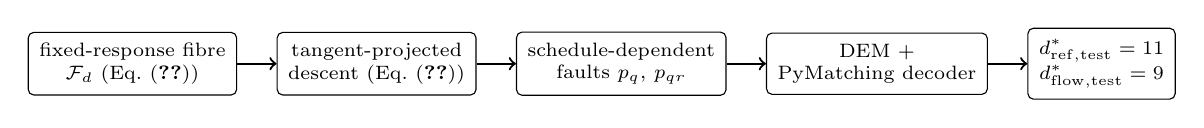
\begin{tikzpicture}[
  box/.style={draw, rounded corners=2pt, align=center, font=\scriptsize, inner sep=4pt},
  arr/.style={->, thick}
]
\node[box] (fibre) {fixed-response fibre\\ \(\F_d\) (Eq.~\eqref{eq:fibre})};
\node[box, right=0.5cm of fibre] (descent) {tangent-projected\\ descent (Eq.~\eqref{eq:general-flow})};
\node[box, right=0.5cm of descent] (faults) {schedule-dependent\\ faults \(p_q,\,p_{qr}\)};
\node[box, right=0.5cm of faults] (dem) {DEM +\\ PyMatching decoder};
\node[box, right=0.5cm of dem] (dist) {\(d_{{\rm ref},\mathrm{test}}^*=11\)\\ \(d_{{\rm flow},\mathrm{test}}^*=9\)};
\draw[arr] (fibre) -- (descent);
\draw[arr] (descent) -- (faults);
\draw[arr] (faults) -- (dem);
\draw[arr] (dem) -- (dist);
\end{tikzpicture}
\caption{Schematic of the audit pipeline (conceptual diagram, not experimental data): schedules on the fixed-response fibre are reshaped by tangent-projected descent, mapped to schedule-dependent faults, decoded through each arm's DEM, and read out as a minimum tested-distance crossover.}
\label{fig:pipeline}
\end{figure}

\subsection{Related work}

Our work contrasts with the main body of surface-code resource estimation. Fowler et al.~\cite{Fowler2012} established the threshold and resource scaling for the standard surface code under uniform depolarizing noise, treating the physical error rate as an exogenous input. More recent code-design efforts, such as the XZZX surface code~\cite{Ataides2021}, improve the threshold by altering the code geometry and stabilizer measurements, while experimental scaling demonstrations (e.g., Google Quantum AI~\cite{Google2023}) focus on validating distance-dependent suppression under a fixed circuit and decoder.

Our contribution is orthogonal: we do not propose a new code, a new decoder, or a calibrated physical noise model; we do not claim this synthetic parameterization as a generally predictive physical noise model. Instead, we target a schedule-level degree of freedom considered here: given a fixed code, decoder family, and noise model, moving within the response fibre reshapes the effective noise correlations seen by the decoder. Dennis et al.~\cite{Dennis2002} already emphasized that correlated errors can materially affect threshold estimates; the present audit asks whether a declared schedule degree of freedom can be optimized against such structure.

\subsection{What the result does not show}

The schedule-to-fault map is synthetic, not derived from a compiler or calibration. The fibre is a declared affine constraint, not unitary equivalence. Decoders are arm-specific (matched pipeline); thus, the results reflect the joint schedule--decoder pipeline, not a schedule effect isolated from decoder adaptation. Only one memory family, one target, five distances, and three frozen seeds are tested. No physical QPU is used.

\subsection{Next falsifiable tests}
\label{sec:next}

Replace the synthetic map with:
\[
  \text{schedule}\to\text{compiled waveform}\to\text{channel}\to\text{Stim DEM}.
\]
Add a fixed-decoder analysis (same DEM or fixed edge weights) to separate schedule effects from decoder adaptation, and a broader noise grid.

An additional control experiment would compare against random feasible walks of equal step count and amplitude variation, starting from the same initial reference. This would separate the design value of the geometric flow from mere sensitivity to schedule perturbation and is a direct next step within the same frozen framework.

\section{Reproducibility}

The standalone source, evidence history, claim boundary, compact reference summary, and file hashes are distributed in the repository
\begin{center}
\url{https://github.com/papasop/quantum}.
\end{center}
The upstream response-fibre geometric-flow project is at
\begin{center}
\url{https://github.com/papasop/Geometric-Flow}.
\end{center}

The repository archives the protocol, compact reference summary, hashes, and claim certificate. The complete compressed Monte Carlo report is archived as results/v0.6.0/report.json.gz; rerunning the audit provides an independent numerical reproduction rather than a byte-identical stochastic artifact. The archived run completed in 478.948 seconds in the reported execution environment; runtime depends on hardware and batch settings. The canonical report certificate SHA-256 before insertion of its self field is
\path{2db9620419ac5a7ff64510c65e0d391c4603b6c361fdd8aadd2d9f96165cbc79}.
The archived compressed report has SHA-256
\path{f9edf8692aaa0f116cc6584507e7f326d184831f251669aa6e2dd2dd143bb95a},
and the claim certificate SHA-256 is
\path{6754415ceb7bb662982c052d2045c7fafced8a7568bf86db7f94a86338a0f00f}.
The full run uses Python 3.12.13, NumPy 2.0.2, Stim 1.16.0, and PyMatching 2.4.0. A quick mode is provided only for pipeline testing and is explicitly ineligible for the prospective claim.

\section{Conclusion}

Within the frozen synthetic schedule-to-fault model, tangent schedule optimization reduced decoded logical failure in all 15 prospective comparisons. Under the frozen Wilson criterion, the minimum tested distance changed from 11 to 9 on all three seeds, corresponding to a 45.34\% reduction in the declared active-coordinate qubit-round proxy. This establishes a numerical mechanism inside the specified model: schedules within the same declared affine response fibre produce different fault exposures, and the geometric flow exploits this to lower the minimum tested distance at fixed reliability. Whether this minimum-tested-distance shift represents a compiler-level resource advantage remains to be tested with compiled waveforms, schedule-dependent physical channels, and calibrated detector error models.

\begin{thebibliography}{99}

\bibitem{Dennis2002}
E.~Dennis, A.~Kitaev, A.~Landahl, and J.~Preskill,
``Topological quantum memory,''
\emph{Journal of Mathematical Physics} \textbf{43}, 4452--4505 (2002).

\bibitem{Fowler2012}
A.~G.~Fowler, M.~Mariantoni, J.~M.~Martinis, and A.~N.~Cleland,
``Surface codes: Towards practical large-scale quantum computation,''
\emph{Physical Review A} \textbf{86}, 032324 (2012).

\bibitem{Ataides2021}
J.~P.~B.~Ataides, D.~K.~Tuckett, S.~D.~Bartlett, S.~T.~Flammia, and B.~J.~Brown,
``The XZZX surface code,''
\emph{Nature Communications} \textbf{12}, 2172 (2021).

\bibitem{Google2023}
Google Quantum AI,
``Suppressing quantum errors by scaling a surface code logical qubit,''
\emph{Nature} \textbf{614}, 676--681 (2023).

\bibitem{Gidney2021}
C.~Gidney,
``Stim: a fast stabilizer circuit simulator,''
\emph{Quantum} \textbf{5}, 497 (2021).

\bibitem{Higgott2022}
O.~Higgott,
``PyMatching: A Python package for decoding quantum codes with minimum-weight perfect matching,''
\emph{ACM Transactions on Quantum Computing} \textbf{3}, 16 (2022).

\bibitem{Wilson1927}
E.~B.~Wilson,
``Probable inference, the law of succession, and statistical inference,''
\emph{Journal of the American Statistical Association} \textbf{22},
209--212 (1927).

\end{thebibliography}

\end{document}